% Phase 2 report, Team T107, Project 21. Generated by report/build_phase2.py from reports/06-10_*.json.
% Edit phase2.tex.tmpl, not phase2.tex.
\documentclass[conference]{IEEEtran}
\usepackage{amsmath,amssymb,graphicx,booktabs,hyperref,xcolor,longtable,array,iftex}
\ifXeTeX\usepackage{fontspec}\setmainfont{texgyretermes}[Extension=.otf,UprightFont=*-regular,BoldFont=*-bold,ItalicFont=*-italic,BoldItalicFont=*-bolditalic]\fi  % tectonic: IEEE's Times (pdflatex/Overleaf already has it)
\graphicspath{{../reports/figures/}{figures/}}
\begin{document}
\title{Flight Delay Prediction at 05:00, Part II: Learned Embeddings, Temporal Deep Learning and an ML + DL Hybrid}
\author{\IEEEauthorblockN{Rishik Chowdary Karuturi, Nakkina Lakshmi Praneeth, Balanagu Sesha Srikar,\\ Shaik Junaid Sami, Siraparapu Shiva Sankar Mani Kanta}
\IEEEauthorblockA{Team T107, Section D, Advanced Machine Learning (Phase 2)\\ Newton School of Technology}}
\maketitle

\begin{abstract}
Phase 1 found that, at a 05:00 decision time, tuned gradient boosting does not beat a regularised logistic regression on NYC 2013 flights. Phase 2 keeps the same label (arrival $\geq$15 min late), decision time, chronological split and single test evaluation, and asks whether deep learning reads the same information better. We build a compact MLP with learned embeddings for carrier, origin and destination; a temporal model in which a GRU reads the last 14 days of delay outcomes, ordered by calendar day and ending on D$-$1; and a hybrid in which a temporal network learns only a correction on top of logistic regression's logit. Every network is tuned with the same leak-free rolling protocol as Phase 1, with epochs in place of trees. On November--December (base rate 0.258) the MLP scores PR AUC 0.425, the temporal model 0.424 and the hybrid 0.417, against 0.403 for logistic regression and 0.386 for Phase 1's XGBoost. All three networks beat logistic regression on the test months, and every paired interval excludes zero (paired day-block bootstrap); the gains are small. The temporal model needs none of the 22 hand-made history features, and removing its GRU costs -0.040. A classical ARIMA model of the daily late rate adds nothing when ranking flights. In an offline what-if, padding the hybrid's flags by 15 minutes avoids 555 late arrivals against 349 for random flights with the same buffer budget.
\end{abstract}

\begin{IEEEkeywords}
flight delay prediction, entity embeddings, GRU, hybrid model, temperature scaling, ablation, ARIMA, what-if analysis
\end{IEEEkeywords}

\section{Introduction}
In Phase 1, logistic regression (test PR AUC 0.403), tuned XGBoost (0.390) and a hybrid that boosts from logistic regression (0.403) were statistically tied. We named three reasons a better model might exist: (i) delay history entered only as hand-made 1/7/28-day averages, which fix the windows and lose the order of days; (ii) tree splits on \emph{absolute} delay-rate levels learned in a high-delay summer misfire in calm autumn months; (iii) carrier, origin and destination were one-hot columns, so rare airports share no strength. The Phase 2 brief (Project 21) asks for a compact MLP with learned embeddings, a temporal model only if history is correctly ordered, a fair comparison at the same decision time, and a calibrated delay-risk model with an offline what-if rescheduling analysis.

\textbf{What stays fixed.} The label, the 05:00 decision time, the 41 Phase 1 features, the chronological split (train Jan 15 -- Aug, validation Sep, calibration Oct, test Nov--Dec) and the rule that the test months are scored once, at the end. Phase 1's three models are refitted in the same run with their reported settings, so Phase 2 is judged against Phase 1 on equal terms. As in Phase 1, the work is five notebooks (06--10), each writing its own module in \texttt{src/fdp/} and its results to \texttt{reports/}, from which every number here is generated.

\section{Related Work}
\textbf{Deep learning for tabular data.} Entity embeddings \cite{guo2016} map each category to a small learned vector, so similar categories share strength; we use them for carrier, origin and destination. Gorishniy et al.\ \cite{gorishniy2021} show that a well-tuned MLP is a strong tabular baseline but that gains over simple models are often small, and Grinsztajn et al.\ \cite{grinsztajn2022} explain why tree ensembles still often beat deep networks on tabular data. We therefore test, rather than assume, that a network helps.

\textbf{Recurrent models.} Gated recurrence fixes the vanishing gradient of plain RNNs \cite{hochreiter1997}; the GRU \cite{cho2014} uses two gates and no separate cell state, so it has fewer weights than an LSTM. Kim et al.\ \cite{kim2016} apply recurrent networks to day-level delay sequences, the closest idea to our temporal input; Gui et al.\ \cite{gui2020} compare an LSTM with a random forest, and Yazdi et al.\ \cite{yazdi2020} train a deep delay model. Like much of this literature, the last two do not restrict inputs to what is known before departure, which our 05:00 rule and leakage tests enforce.

\textbf{Training and calibration.} We regularise with dropout \cite{srivastava2014} and decoupled weight decay (AdamW \cite{loshchilov2019}, built on Adam \cite{kingma2015}). Guo et al.\ \cite{guo2017} show that modern networks are often over-confident and that one-parameter temperature scaling fixes much of it; we compare it with Platt scaling \cite{platt1999}, the method of Phase 1.

\textbf{Time series.} ARIMA \cite{box2015} is the classical model for one series. Our daily late rate is such a series, but the task is to rank flights within each day; we measure what ARIMA adds.

\section{Data for Deep Learning}
\subsection{Tabular Inputs}
A network needs scaled numbers and category indices. The 41 Phase 1 features are median-imputed and z-scored with statistics from the training rows, plus one flag for a missing aircraft record (42 inputs). Gradient descent moves every weight with similar step sizes, so unscaled inputs make training slow and unstable. Each category gets an index: 0 for never seen in training, 1 for seen fewer than 50 times, 2 and up for common ones, so a new airport in November gets its own learned ``unknown'' vector instead of crashing. The embedding size grows slowly with the number of categories, $\min(16, \mathrm{round}(1.6\,n^{0.56}))$ (Table~\ref{tab:inputs}).

\begin{table}[t]\centering\caption{Category inputs: embedding vs one-hot width.}\label{tab:inputs}
\footnotesize\begin{tabular}{lcccc}\toprule
Column & In training & Table rows & Embedding & One-hot\\\midrule
carrier & 16 & 17 & 8 & 17\\
origin & 3 & 5 & 4 & 5\\
dest & 102 & 94 & 16 & 94\\
\bottomrule\end{tabular}\end{table}

\subsection{Ordered Delay Histories}
The brief allows a temporal model only if history is correctly ordered. For a flight on day $D$ we build a sequence over days $t = D-14, \dots, D-1$ with 16 channels: the overall NYC late rate $p_t$ and log volume, and for six groups $g$ (origin, carrier, carrier at origin, route, flight number, aircraft) a smoothed rate \emph{relative} to that day's overall rate and the group's log volume,
\begin{equation}
\tilde r_{g,t} = \frac{k_{g,t} + \alpha\, p_t}{n_{g,t} + \alpha} - p_t,\qquad \alpha = 5.0,
\end{equation}
plus the weekday of $t$ (sin/cos). $k_{g,t}$ and $n_{g,t}$ are the late and labelled flights of group $g$ on day $t$. Days before the data start are zero. The training sequences take 184.3 MB (float32). Fig.~\ref{fig:seq} shows one flight's two weeks.

\textbf{Leakage test.} A unit test flips every label from a cut-off day onward: the sequences for that day must be identical, and to show the test can fail, the next day's must change. It passes, as do the two Phase 1 leakage tests.

\begin{figure}[t]\centering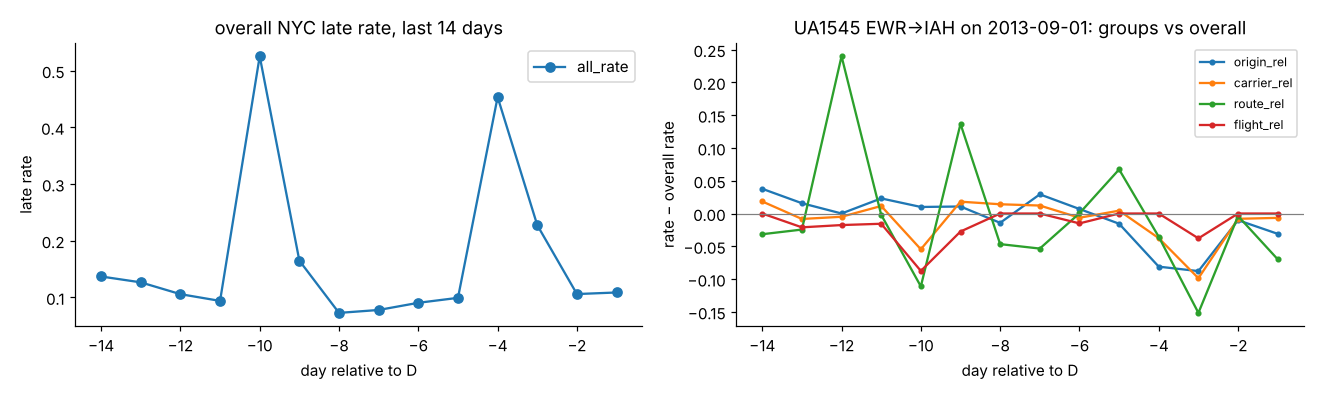
\includegraphics[width=\columnwidth]{06_one_sequence.png}
\caption{One flight's 14-day input sequence, as the GRU reads it.}\label{fig:seq}\end{figure}

\subsection{Why Relative Rates: Drift on the Inputs}
Phase 1 blamed tree splits on absolute levels for boosting's autumn drop. We measure it on the inputs: a rule written in July, ``origin's 7-day rate in July's top quarter'', is applied to every month (Table~\ref{tab:drift}). On the absolute rate it fires on 0.00--0.27 of flights and on none in September--November; on the relative rate it fires on 0.05--0.36 in every month. A relative rate asks ``worse than everyone else right now?'', which means the same in every season.

\begin{table*}[t]\centering\caption{Share of flights flagged by a July rule ``origin 7-day rate in the top quarter'', by month.}\label{tab:drift}
\footnotesize\begin{tabular}{lcccccccccccc}\toprule
Rule written on & 1 & 2 & 3 & 4 & 5 & 6 & 7 & 8 & 9 & 10 & 11 & 12\\\midrule
absolute & 0.00 & 0.00 & 0.00 & 0.17 & 0.00 & 0.04 & 0.24 & 0.06 & 0.00 & 0.00 & 0.00 & 0.27\\
relative & 0.36 & 0.20 & 0.29 & 0.28 & 0.19 & 0.12 & 0.24 & 0.14 & 0.05 & 0.19 & 0.16 & 0.24\\
\bottomrule\end{tabular}\end{table*}

\subsection{A Classical Time-Series Check: ARIMA}
The daily late rate is a time series (Phase 1's ACF, PACF and ADF test chose our lag windows), so we fit ARIMA \cite{box2015} on days up to 2013-08-31 and judge one-step-ahead forecasts on September and October (mean daily late rate 0.138 and 0.174; Table~\ref{tab:arima}). ARIMA(0,1,1), which is exponential smoothing and follows a drifting level, forecasts best of the four, yet ``yesterday's rate'' is as good or better (MAE 0.079 in September).

ARIMA gives one number per day, so it cannot rank the roughly 900 flights within a day. Measured on the rolling months, with parameters refitted before each scored month (Table~\ref{tab:arimarank}): ARIMA(1,0,1)'s forecast used alone scores 0.3081, against 0.4092 for logistic regression; added as a feature it changes logistic regression by -0.0004, because it correlates 0.96 with the ``yesterday's overall rate'' feature already in the model. Knowing the day's level does not separate flights; the GRU below is our time-series model.

\begin{table}[t]\centering\caption{One-step forecasts of the daily late rate (MAE).}\label{tab:arima}
\footnotesize\begin{tabular}{lccc}\toprule
Forecast & AIC & MAE Sep & MAE Oct\\\midrule
ARIMA(1, 0, 0) & -272.0 & 0.119 & 0.093\\
ARIMA(1, 0, 1) & -272.9 & 0.123 & 0.094\\
ARIMA(2, 0, 1) & -270.9 & 0.123 & 0.094\\
ARIMA(0, 1, 1) & -239.5 & 0.096 & 0.060\\
yesterday's rate & -- & 0.079 & 0.079\\
mean of the last 7 days & -- & 0.094 & 0.067\\
training mean (no memory) & -- & 0.162 & 0.113\\
\bottomrule\end{tabular}\end{table}

\begin{table}[t]\centering\caption{ARIMA as a score and as a feature (rolling-month mean PR AUC). Corr.: with yesterday's-rate feature.}\label{tab:arimarank}
\setlength{\tabcolsep}{3pt}\footnotesize\begin{tabular}{lccccc}\toprule
Order & Alone & LR & LR + ARIMA & Gain & Corr.\\\midrule
ARIMA(1, 0, 1) & 0.3081 & 0.4092 & 0.4088 & -0.0004 & 0.96\\
ARIMA(0, 1, 1) & 0.2363 & 0.4092 & 0.4075 & -0.0017 & 0.55\\
\bottomrule\end{tabular}\end{table}

\section{Method}
\subsection{MLP with Learned Embeddings}
The numeric block $x$ and the three embedding vectors $e_c, e_o, e_d$ are concatenated into $h_0 = [x; e_c; e_o; e_d]$, passed through two Linear--ReLU--Dropout layers, and mapped to one logit:
\begin{equation}
h_\ell = \mathrm{Dropout}\big(\mathrm{ReLU}(W_\ell h_{\ell-1} + b_\ell)\big),\qquad z = w^\top h_2 + b.
\end{equation}
The loss is log loss, $-\big(y\log\sigma(z) + (1-y)\log(1-\sigma(z))\big)$, minimised by back-propagation with mini-batch AdamW. Logistic regression is the same model with no hidden layer, which makes the comparison clean. ReLU adds the non-linearity (stacked linear layers collapse into one); dropout stops units from co-adapting; weight decay is the network version of the L2 penalty $C$. The chosen network has 52,861 weights, 1,660 of them in the embeddings.

\subsection{Temporal Model: a GRU over 14 Days}
A GRU \cite{cho2014} reads the sequence oldest day first, keeping a hidden state $h_t$ (32 numbers):
\begin{gather}
u_t = \sigma(W_u s_t + U_u h_{t-1}),\quad r_t = \sigma(W_r s_t + U_r h_{t-1}),\\
\tilde h_t = \tanh\big(W s_t + U(r_t \odot h_{t-1})\big),\quad h_t = (1-u_t)\odot h_{t-1} + u_t \odot \tilde h_t .
\end{gather}
The update gate $u_t$ decides how much of today replaces the memory; the reset gate $r_t$ how much old memory is used when reading today. The last state joins $h_0$ of the MLP. The same weights read every day, so the model learns how to weigh recent and older days instead of us fixing 1/7/28-day windows. With 14 short steps and 16 channels a GRU is enough; an LSTM has more weights and a Transformer's long-range attention is not needed for two weeks. ``Temporal: GRU replaces hand history'' drops the 22 hand-made history features and keeps the 19 others, the direct test of whether a network can learn from raw ordered days what Phase 1 engineered by hand.

\subsection{Hybrid: Logistic Regression + Temporal Correction}
\begin{equation}
z(x) = \underbrace{w^\top x + b}_{\text{LR, fixed, 41 features}} + \underbrace{g_\theta\big(x_{\setminus\text{hist}}, e, \mathrm{GRU}(s)\big)}_{\text{network: correction}} .
\end{equation}
Logistic regression is fitted first and its logit enters as a fixed offset. The network's last layer starts at zero, so before training the hybrid \emph{is} logistic regression, and early stopping also scores this ``epoch 0'', so if no correction transfers it keeps plain logistic regression. Each part has a job: logistic regression is Phase 1's most season-stable model, the network adds interactions and ordered history. It is the deep-learning version of Phase 1's boosting-from-LR hybrid.

\subsection{Training Protocol and Calibration}
Epochs play the role of trees. For each rolling month $m \in \{\text{Jul}, \text{Aug}, \text{Sep}\}$: train on months before $m-1$ and early-stop on $m-1$ by PR AUC (patience 3), refit on all months before $m$ for that many epochs, score $m$. Early-stopping on the scored month is the trap Phase 1 measured. The final epoch count is the median over folds. Calibration: temperature scaling $p = \sigma(z/T)$ \cite{guo2017} or Platt scaling $p=\sigma(az+b)$ \cite{platt1999}, judged by expected calibration error, $\mathrm{ECE} = \sum_b \frac{|B_b|}{N}\,|\bar y_b - \bar p_b|$ over probability bins $B_b$. Both leave the ranking, so PR AUC, unchanged.

\section{Experiments}
\subsection{Over-fitting and the MLP Search}
Without early stopping or dropout the training loss falls every epoch while September's PR AUC peaks at epoch 4 (0.2735) and then declines (Fig.~\ref{fig:overfit}). A random search over size, dropout, learning rate and weight decay, scored with the honest protocol, found settings within 0.0032 of each other (Table~\ref{tab:search}); the best, (256, 128) units, dropout 0.5, learning rate 0.0003, weight decay 0.01, reached 0.4064, still below logistic regression's 0.4092. Its body is reused by every network below. The first principal component of the learned destination embeddings correlates only 0.01 with the airports' training late rate: the destination's own rate is already in the history features, so we do not claim the embeddings found a ``delay axis''.

\begin{figure}[t]\centering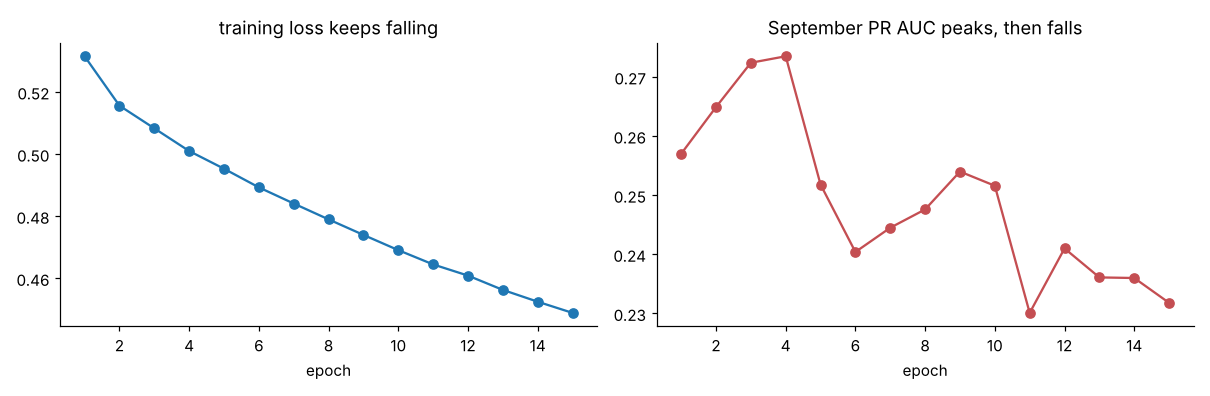
\includegraphics[width=\columnwidth]{07_overfitting.png}
\caption{No early stopping, no dropout: training loss falls, September PR AUC peaks early.}\label{fig:overfit}\end{figure}

\begin{table}[t]\centering\caption{MLP search (rolling-month mean PR AUC).}\label{tab:search}
\setlength{\tabcolsep}{3pt}\footnotesize\begin{tabular}{lccccc}\toprule
Hidden & Drop. & LR & WD & Mean & Epochs/fold\\\midrule
256-128 & 0.5 & 0.0003 & 0.01 & 0.4064 & [8,12,2]\\
256-128 & 0.2 & 0.001 & 0.0001 & 0.4063 & [2,1,1]\\
64-32 & 0.2 & 0.0003 & 0.01 & 0.4045 & [13,8,3]\\
64-32 & 0.2 & 0.0003 & 0.0001 & 0.4044 & [13,8,3]\\
256-128 & 0.5 & 0.001 & 0.01 & 0.4043 & [4,4,1]\\
64-32 & 0.5 & 0.001 & 0.01 & 0.4041 & [4,8,2]\\
64-32 & 0.5 & 0.001 & 0.0001 & 0.4039 & [6,8,2]\\
256-128 & 0.2 & 0.001 & 0.01 & 0.4032 & [2,2,1]\\
\bottomrule\end{tabular}\end{table}

\subsection{All Models on the Same Rolling Months}
Table~\ref{tab:roll} and Fig.~\ref{fig:roll} compare every candidate on the same honest folds. Phase 1's XGBoost rows come from the Phase 1 report, which used the same months and protocol. The temporal model with \emph{no} hand-made history scores 0.4111, above the GRU that also gets the 22 history features (0.4086), and the hybrid scores 0.4155 against 0.4092 for logistic regression. The temporal models also choose longer, steadier epoch counts than the MLP.

\begin{table}[t]\centering\caption{Rolling-month PR AUC (each month scored by a model that never saw it).}\label{tab:roll}
\setlength{\tabcolsep}{2.5pt}\footnotesize\begin{tabular}{lccccc}\toprule
Model & Jul & Aug & Sep & Mean & Epochs\\\midrule
Logistic regression & 0.5565 & 0.4055 & 0.2655 & 0.4092 & --\\
MLP + embeddings & 0.5598 & 0.4036 & 0.2553 & 0.4062 & [6,8,2]\\
GRU + all features & 0.5635 & 0.4029 & 0.2593 & 0.4086 & [8,7,2]\\
GRU, no hand history & 0.5652 & 0.4047 & 0.2633 & 0.4111 & [16,19,11]\\
Hybrid: LR + GRU & 0.5658 & 0.4102 & 0.2704 & 0.4155 & [11,15,11]\\
XGBoost (P1 report) & 0.5480 & 0.3910 & 0.2190 & 0.3860 & --\\
XGB from LR (P1 report) & 0.5590 & 0.3910 & 0.2680 & 0.4060 & --\\
\bottomrule\end{tabular}\end{table}

\begin{figure}[t]\centering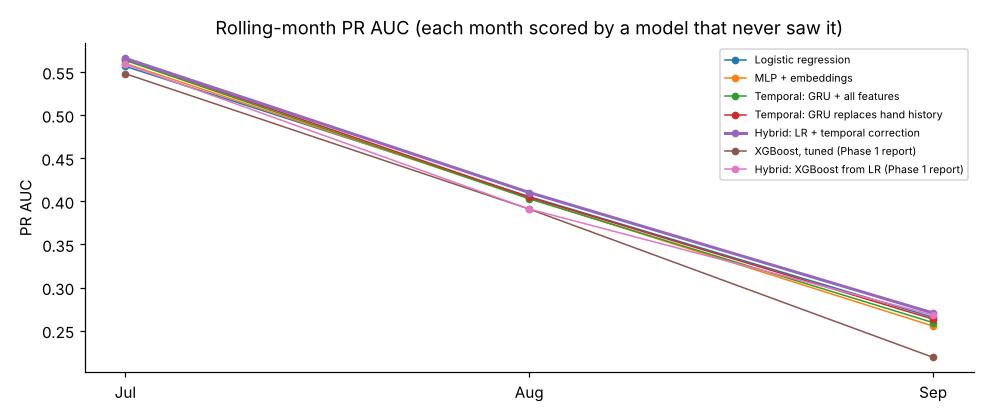
\includegraphics[width=\columnwidth]{08_rolling.png}
\caption{Rolling-month PR AUC of every candidate.}\label{fig:roll}\end{figure}

\subsection{Seeds}
A network's score moves with its random start. We re-ran the three test candidates with two more seeds (Table~\ref{tab:seeds}). The decision rule, fixed before the test, was that a network counts as ahead of logistic regression only if \emph{every} seed is above its mean (0.4092). The hybrid meets it.

\begin{table}[t]\centering\caption{Rolling-month mean per seed (42, 1, 2).}\label{tab:seeds}
\setlength{\tabcolsep}{3pt}\footnotesize\begin{tabular}{lp{1.25in}cc}\toprule
Model & Per seed & Mean & Range\\\midrule
MLP & 0.4062, 0.4079, 0.4076 & 0.4072 & 0.0017\\
Temporal & 0.4111, 0.4106, 0.4081 & 0.4099 & 0.0030\\
Hybrid & 0.4155, 0.4142, 0.4132 & 0.4143 & 0.0023\\
\bottomrule\end{tabular}\end{table}

\subsection{Ablation}
Seven variants of the temporal model, one change each, same protocol and seed (Table~\ref{tab:ablation}, Fig.~\ref{fig:ablation}), read against the full model's seed range (0.0030). Removing the GRU branch costs -0.0400; every other change, including adding back the hand-made history, moves the mean by no more than about the seed range. Relative rates, the idea motivated by the drift table, made no measurable difference (+0.0007 with absolute rates): the GRU also sees the overall rate as its own channel and can learn the difference itself. We report that this idea did not pay off here.

\begin{table}[t]\centering\caption{Ablation of the temporal model (rolling-month mean PR AUC).}\label{tab:ablation}
\setlength{\tabcolsep}{3pt}\footnotesize\begin{tabular}{lccc}\toprule
Variant & Mean & $\Delta$ vs full & Epochs\\\midrule
full model & 0.4111 & +0.0000 & [16,19,11]\\
+ hand-made history (22 features) & 0.4086 & -0.0025 & [8,7,2]\\
$-$ GRU branch (MLP, no history) & 0.3710 & -0.0400 & [19,15,2]\\
absolute rates in the sequence & 0.4117 & +0.0007 & [11,5,11]\\
one-hot instead of embeddings & 0.4079 & -0.0032 & [13,14,6]\\
7-day sequence & 0.4090 & -0.0020 & [16,19,9]\\
no dropout, no weight decay & 0.4094 & -0.0017 & [8,8,6]\\
no early stopping (15 epochs) & 0.4107 & -0.0004 & [15,15,15]\\
\bottomrule\end{tabular}\end{table}

\begin{figure}[t]\centering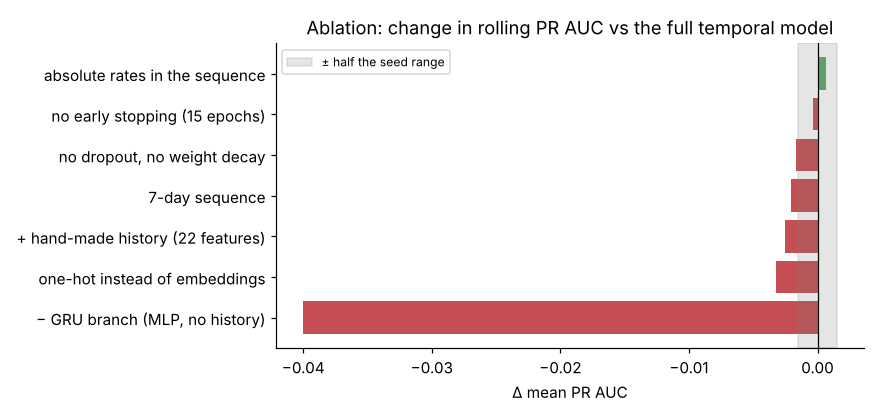
\includegraphics[width=\columnwidth]{09_ablation.png}
\caption{Ablation: change in rolling PR AUC; grey band = $\pm$ half the seed range.}\label{fig:ablation}\end{figure}

\subsection{Choosing the Calibration Method}
Models were trained on January 15 -- August, calibrators fitted on September (late rate 0.137) and judged on October (0.176), so the test months stay closed (Table~\ref{tab:calib}). Every fitted temperature is below 1 (0.716--0.786): unlike the deep image networks of Guo et al., our small, regularised, early-stopped networks were under-confident, so their logits are sharpened, not softened. Temperature had the lower mean October ECE and is used for every model in the final evaluation, fitted on October. Platt's intercept copies the calibration month's base rate, which hurts when the base rate moves (0.137 $\rightarrow$ 0.176 $\rightarrow$ 0.258).

\begin{table}[t]\centering\caption{Calibration on October (ECE): fitted on September.}\label{tab:calib}
\setlength{\tabcolsep}{3pt}\footnotesize\begin{tabular}{lcccc}\toprule
Model & $T$ & Raw & Temperature & Platt\\\midrule
LR & 0.716 & 0.041 & 0.026 & 0.037\\
MLP & 0.734 & 0.036 & 0.029 & 0.035\\
Temporal & 0.786 & 0.046 & 0.036 & 0.029\\
Hybrid & 0.739 & 0.041 & 0.030 & 0.036\\
\bottomrule\end{tabular}\end{table}

\section{Results}
\subsection{The Test Months, Scored Once}
Every model is refitted on January 15 -- September 30 (networks for the median fold epochs: the MLP 6, the temporal model 16, the hybrid 11), temperature-scaled on October, and scored once on November--December (Table~\ref{tab:test}, Fig.~\ref{fig:test}). Because two models' separate intervals share the day-to-day noise, we also bootstrap the \emph{difference} against logistic regression on the same resampled days (a paired day-block bootstrap, 200 resamples): $\Delta^{(b)} = \mathrm{AP}_{\text{model}}(B_b) - \mathrm{AP}_{\text{LR}}(B_b)$.

All three networks beat logistic regression on the test months, and every paired interval excludes zero: the MLP by +0.022 [+0.004, +0.036], the temporal model by +0.021 [+0.002, +0.037] and the hybrid by +0.014 [+0.002, +0.028]. Phase 1's XGBoost is 0.017 below logistic regression with an interval that contains zero, and Phase 1's hybrid matches it (+0.001 [-0.003, +0.004]), reproducing Phase 1's finding. Our XGBoost refit scores 0.386 against 0.390 in the Phase 1 report, a third-decimal library and run difference; logistic regression matches. The networks also keep more lift in November (1.56/1.61/1.64 for MLP/temporal/hybrid vs 1.36 for XGBoost), the month Phase 1's trees lost most.

\textbf{Calibration on the test months.} Temperature scaling fitted on October lowered the test ECE for the MLP and raised it for logistic regression, Phase 1's XGBoost, Phase 1's XGBoost hybrid, the temporal model and the hybrid. The base rate rose from 0.176 to 0.258, and a calibrator fitted in one month cannot know that; we report this honestly rather than re-fitting on the test.

\begin{table*}[t]\centering\caption{Test results, Nov--Dec 2013 (base rate 0.258), scored once. 95\% CI: day-block bootstrap. $\Delta$ vs LR: paired day-block bootstrap of the difference. ECE: raw $\rightarrow$ after temperature scaling.}\label{tab:test}
\footnotesize\begin{tabular}{lccccccc}\toprule
Model & PR AUC & 95\% CI & $\Delta$ vs LR [95\% CI] & ROC AUC & Lift & Brier & ECE\\\midrule
Majority class & 0.258 & -- & -- & 0.500 & 1.00 & 0.192 & 0.010\\
Rule: flight's 28-day delay rate & 0.369 & -- & -- & 0.638 & 1.43 & 0.184 & 0.036\\
Logistic regression & 0.403 & [0.351, 0.459] & -- & 0.670 & 1.56 & 0.180 & 0.029 $\rightarrow$ 0.034\\
XGBoost (Phase 1) & 0.386 & [0.332, 0.447] & -0.017 [-0.046, +0.013] & 0.653 & 1.49 & 0.183 & 0.033 $\rightarrow$ 0.046\\
Hybrid: XGBoost from LR (Phase 1) & 0.404 & [0.352, 0.460] & +0.001 [-0.003, +0.004] & 0.670 & 1.56 & 0.179 & 0.028 $\rightarrow$ 0.030\\
MLP + embeddings & 0.425 & [0.363, 0.483] & +0.022 [+0.004, +0.036] & 0.681 & 1.65 & 0.176 & 0.032 $\rightarrow$ 0.018\\
Temporal: GRU replaces hand history & 0.424 & [0.360, 0.480] & +0.021 [+0.002, +0.037] & 0.686 & 1.64 & 0.178 & 0.029 $\rightarrow$ 0.041\\
Hybrid: LR + temporal correction & 0.417 & [0.364, 0.471] & +0.014 [+0.002, +0.028] & 0.684 & 1.62 & 0.177 & 0.033 $\rightarrow$ 0.035\\
\bottomrule\end{tabular}\end{table*}

\begin{figure}[t]\centering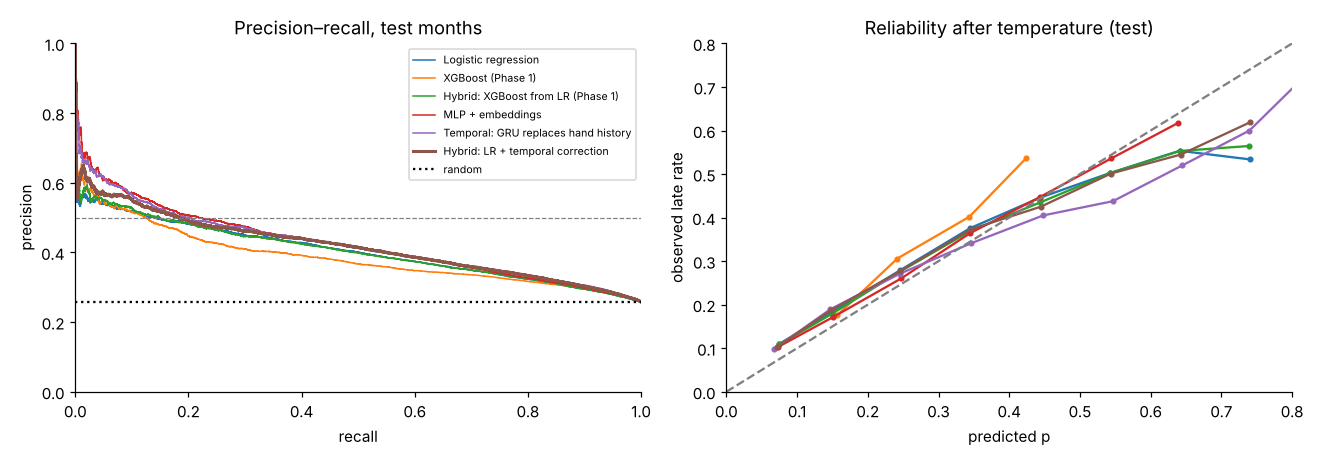
\includegraphics[width=\columnwidth]{10_test_pr_reliability.png}
\caption{Test precision--recall curves and reliability after temperature scaling.}\label{fig:test}\end{figure}

\subsection{Recall at the Operational Precision Rule}
The brief asks for recall at a selected operational precision threshold. The rule was chosen in Phase 1, before any test score: flag a flight when its calibrated probability is $\geq 0.5$, rule (b). Rule (a), a score cut-off fixed on October for precision 0.5, is shown for comparison (Table~\ref{tab:biz}). Under rule (b) the hybrid flags 66.0 flights per 1,000 at precision 0.526 and recall 0.135, against 49.8, 0.519 and 0.100 for logistic regression. Two rows are empty by construction: temperature has no intercept, so Phase 1's XGBoost, whose probabilities stay near the base rate, never reaches $p \geq 0.5$; and for the hybrid no October cut-off reaches precision 0.5. Both are real outcomes of rules fixed in advance.

\begin{table}[t]\centering\caption{Flag list per 1,000 test flights: (a) October cut-off, (b) calibrated $p\geq0.5$.}\label{tab:biz}
\setlength{\tabcolsep}{2pt}\footnotesize\begin{tabular}{llccccc}\toprule
Model & Rule & Prec. & Recall & Flagged & Late & Random\\\midrule
LR & (a) & 0.538 & 0.055 & 26.4 & 14.2 & 6.8\\
LR & (b) & 0.519 & 0.100 & 49.8 & 25.9 & 12.9\\
XGBoost (P1) & (a) & 0.530 & 0.066 & 31.9 & 16.9 & 8.2\\
XGBoost (P1) & (b) & 0.000 & 0.000 & 0.0 & 0.0 & 0.0\\
XGB from LR (P1) & (a) & 0.548 & 0.055 & 26.0 & 14.2 & 6.7\\
XGB from LR (P1) & (b) & 0.521 & 0.105 & 51.9 & 27.0 & 13.4\\
MLP & (a) & 0.624 & 0.046 & 18.9 & 11.8 & 4.9\\
MLP & (b) & 0.565 & 0.109 & 49.7 & 28.1 & 12.8\\
Temporal & (a) & 0.637 & 0.027 & 10.9 & 6.9 & 2.8\\
Temporal & (b) & 0.491 & 0.212 & 111.8 & 54.9 & 28.9\\
Hybrid & (a) & 0.000 & 0.000 & 0.0 & 0.0 & 0.0\\
Hybrid & (b) & 0.526 & 0.135 & 66.0 & 34.7 & 17.1\\
\bottomrule\end{tabular}\end{table}

\section{What-If Rescheduling}
\textbf{Rule.} At 05:00, add a buffer of $B$ minutes to the scheduled arrival of every flight the model flags. \textbf{Assumptions.} (A1) Padding moves the published arrival time, not the landing, so a padded flight is late only if $\text{arr\_delay} - B \geq 15$. (A2) No knock-on effects on the aircraft's next flight, crews, gates or connections. (A3) The cost is the buffer minutes added, and every policy gets the same budget; a minute is ``used'' if the flight was at least that late. (A4) Actual test-month delays only score the policy offline; the flags use 05:00 information only, as test labels score a model. (A5) Cancelled and diverted flights have no arrival time and are left out.

\textbf{Same budget, four policies.} The budget is the hybrid's rule-(b) flag count, 3,565 of 53,991 test flights, $\times$ 15 minutes. Each score pads its own top 3,565 flights; random flights (mean of 200 draws) are the floor (Table~\ref{tab:policy}). The hybrid's flags avoid 555 late arrivals, logistic regression's 546, the planner's 28-day rule 528 and random flights 349; 62.5\% of the hybrid's buffer minutes are used, against 34.3\% for random flags. The gap to random is the value the risk score adds; the gap between the models is small, as in the test table.

\textbf{Buffer size.} Larger buffers avoid more late arrivals but each extra minute buys less (Table~\ref{tab:sweep}, Fig.~\ref{fig:whatif}): 207 avoided at 5 minutes, 1313 at 60, while 1,689 padded flights would have been on time anyway at every buffer size.

\begin{table}[t]\centering\caption{Same budget (3,565 flights $\times$ 15 min), test months.}\label{tab:policy}
\setlength{\tabcolsep}{2.5pt}\footnotesize\begin{tabular}{lcccc}\toprule
Policy & Avoided & Per 1,000 & Of all late & Minutes used\\\midrule
hybrid flags & 555 & 10.28 & 4.0\% & 62.5\%\\
logistic regression flags & 546 & 10.11 & 3.9\% & 60.5\%\\
planner rule (28-day rate) & 528 & 9.78 & 3.8\% & 54.8\%\\
random flights & 349 & 6.47 & 2.5\% & 34.3\%\\
\bottomrule\end{tabular}\end{table}

\begin{table}[t]\centering\caption{Buffer sweep on the hybrid's flags.}\label{tab:sweep}
\setlength{\tabcolsep}{2.5pt}\footnotesize\begin{tabular}{cccccc}\toprule
$B$ & Avoided & Still late & On time anyway & Per 1,000 min & Used\\\midrule
5 & 207 & 1669 & 1689 & 11.6 & 70.0\%\\
10 & 391 & 1485 & 1689 & 11.0 & 66.2\%\\
15 & 555 & 1321 & 1689 & 10.4 & 62.5\%\\
20 & 687 & 1189 & 1689 & 9.6 & 59.2\%\\
30 & 919 & 957 & 1689 & 8.6 & 53.3\%\\
45 & 1149 & 727 & 1689 & 7.2 & 46.0\%\\
60 & 1313 & 563 & 1689 & 6.1 & 40.3\%\\
\bottomrule\end{tabular}\end{table}

\begin{figure}[t]\centering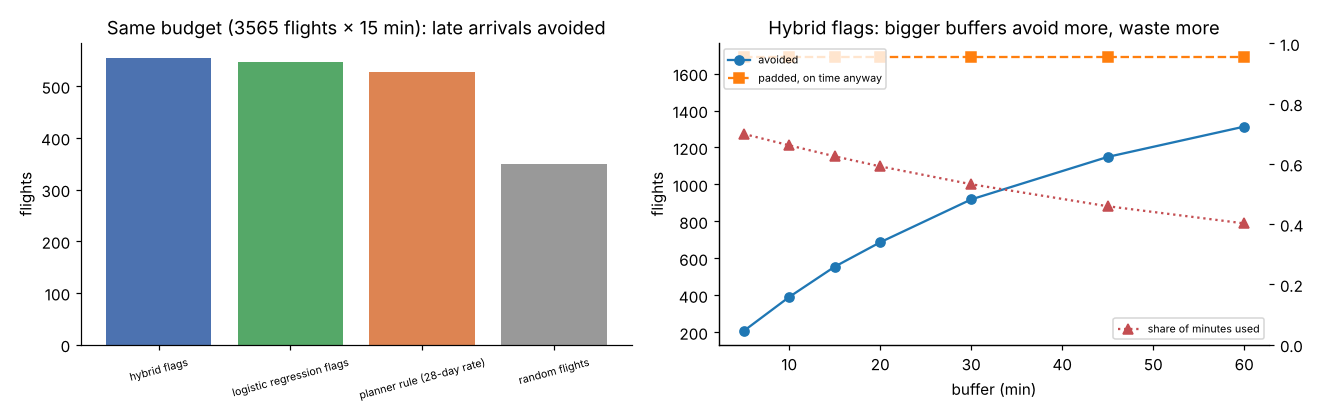
\includegraphics[width=\columnwidth]{10_rescheduling.png}
\caption{Left: late arrivals avoided with the same budget. Right: the buffer trade-off on the hybrid's flags.}\label{fig:whatif}\end{figure}

\section{Threats to Validity}
(i) One year of data cannot separate season from trend, and the test months (with the holiday peak) behave differently from July--September: the rolling months favoured only the hybrid, while the test months favour all three networks. We report both. (ii) The rolling months were used for every selection (MLP search, model choice, ablation), so rolling means are slightly optimistic; the test set is unaffected. (iii) Seeds move rolling means by up to 0.0030, the same size as several of the differences we discuss. (iv) Temperature fitted on October helped some models and hurt others under the base-rate shift. (v) Our XGBoost refit differs from the Phase 1 report in the third decimal. (vi) The what-if ignores knock-on effects through the aircraft rotation and crews, prices every buffer minute equally, and only pads arrivals.

\section{Conclusion}
At a 05:00 decision time, deep learning reads the same information slightly better than logistic regression: on the test months the MLP (0.425), the temporal model (0.424) and the hybrid (0.417) all lie above logistic regression (0.403) and Phase 1's XGBoost (0.386), but the gains are small, about two hundredths of PR AUC. The most interesting finding is that a GRU over raw, ordered daily outcomes replaces all 22 hand-made history features, and that the GRU is the one component whose removal clearly hurts. The model we would deploy is the hybrid: it was the only network ahead of logistic regression in every seed on the rolling months, it is significantly above it on the test months (+0.014 [+0.002, +0.028]), and by construction it falls back to logistic regression. The MLP scored highest on the test months, but choosing it now would be choosing on the test set. Future work: weather forecasts known at 05:00, several years of data, and an aircraft-rotation model so the what-if can include knock-on effects.

\section*{Contributions}
\textbf{Balanagu Sesha Srikar}: deep-learning inputs, ordered 14-day histories, the sequence leakage test, the drift measurement and the ARIMA module (notebook 06, \texttt{dl\_inputs.py}, \texttt{timeseries.py}). \textbf{Siraparapu Shiva Sankar Mani Kanta}: the MLP with embeddings, training loop, honest epoch protocol and search (notebook 07, \texttt{deep.py}). \textbf{Rishik Chowdary Karuturi}: the temporal model, the hybrid, the rolling comparison, seeds and Phase 1 refits (notebook 08, \texttt{phase1\_models.py}). \textbf{Nakkina Lakshmi Praneeth}: ablation studies and calibration (notebook 09, \texttt{calibration.py}). \textbf{Shaik Junaid Sami}: final evaluation, paired tests, operational metrics and the what-if rescheduling analysis (notebook 10, \texttt{rescheduling.py}); the ARIMA experiment (\texttt{report/arima\_check.py}) and this report.

\begin{thebibliography}{99}\footnotesize
\bibitem{guo2017} C.~Guo, G.~Pleiss, Y.~Sun and K.~Q.~Weinberger, ``On calibration of modern neural networks,'' in \emph{Proc.\ ICML}, 2017, pp.~1321--1330.
\bibitem{guo2016} C.~Guo and F.~Berkhahn, ``Entity embeddings of categorical variables,'' arXiv:1604.06737, 2016.
\bibitem{hochreiter1997} S.~Hochreiter and J.~Schmidhuber, ``Long short-term memory,'' \emph{Neural Computation}, vol.~9, no.~8, pp.~1735--1780, 1997.
\bibitem{cho2014} K.~Cho \emph{et al.}, ``Learning phrase representations using RNN encoder--decoder for statistical machine translation,'' in \emph{Proc.\ EMNLP}, 2014, pp.~1724--1734.
\bibitem{srivastava2014} N.~Srivastava, G.~Hinton, A.~Krizhevsky, I.~Sutskever and R.~Salakhutdinov, ``Dropout: a simple way to prevent neural networks from overfitting,'' \emph{JMLR}, vol.~15, pp.~1929--1958, 2014.
\bibitem{loshchilov2019} I.~Loshchilov and F.~Hutter, ``Decoupled weight decay regularization,'' in \emph{Proc.\ ICLR}, 2019.
\bibitem{kingma2015} D.~P.~Kingma and J.~Ba, ``Adam: a method for stochastic optimization,'' in \emph{Proc.\ ICLR}, 2015.
\bibitem{gorishniy2021} Y.~Gorishniy, I.~Rubachev, V.~Khrulkov and A.~Babenko, ``Revisiting deep learning models for tabular data,'' in \emph{Proc.\ NeurIPS}, 2021.
\bibitem{grinsztajn2022} L.~Grinsztajn, E.~Oyallon and G.~Varoquaux, ``Why do tree-based models still outperform deep learning on typical tabular data?,'' in \emph{NeurIPS Datasets and Benchmarks}, 2022.
\bibitem{kim2016} Y.~J.~Kim, S.~Choi, S.~Briceno and D.~Mavris, ``A deep learning approach to flight delay prediction,'' in \emph{Proc.\ IEEE/AIAA DASC}, 2016.
\bibitem{gui2020} G.~Gui, F.~Liu, J.~Sun, J.~Yang, Z.~Zhou and D.~Zhao, ``Flight delay prediction based on aviation big data and machine learning,'' \emph{IEEE Trans.\ Vehicular Technology}, vol.~69, no.~1, pp.~140--150, 2020.
\bibitem{yazdi2020} M.~F.~Yazdi, S.~R.~Kamel, S.~J.~M.~Chabok and M.~Kheirabadi, ``Flight delay prediction based on deep learning and Levenberg--Marquardt algorithm,'' \emph{J.\ Big Data}, vol.~7, 2020.
\bibitem{box2015} G.~E.~P.~Box, G.~M.~Jenkins, G.~C.~Reinsel and G.~M.~Ljung, \emph{Time Series Analysis: Forecasting and Control}, 5th ed., Wiley, 2015.
\bibitem{platt1999} J.~Platt, ``Probabilistic outputs for support vector machines and comparisons to regularized likelihood methods,'' in \emph{Advances in Large Margin Classifiers}, MIT Press, 1999.
\end{thebibliography}

\onecolumn
\section*{Appendix: Decision Log}
One line per design decision (NB = notebook); the reasons are in the sections above.
\footnotesize
\begin{longtable}{@{}r c >{\raggedright\arraybackslash}p{3.0in} >{\raggedright\arraybackslash}p{3.2in}@{}}
\toprule
\# & NB & Decision & Outcome\\\midrule\endhead
1 & 06 & Same label, 05:00 decision time, split and test-once rule as Phase 1 & Phase 2 is judged against Phase 1 on equal terms\\
2 & 06 & z-score numeric block + missing-aircraft flag, fitted on training rows & 41 features + 1 flag = 42 inputs\\
3 & 06 & Category indices: 0 unknown, 1 rare ($<$50), 2... common & Embedding sizes 8 / 4 / 16 (carrier / origin / dest)\\
4 & 06 & Ordered 14-day histories ending on D$-$1, 16 channels & Sequence leakage test passes\\
5 & 06 & History stored relative to the day's overall rate & July rule fires 0.051--0.365 (relative) vs 0.000--0.270 (absolute)\\
6 & 06 & ARIMA measured as forecaster, score and feature & Alone 0.308 vs LR 0.409; as a feature -0.0004\\
7 & 07 & Compact MLP, learned embeddings, log loss & 52,861 weights, 1,660 in embeddings\\
8 & 07 & Dropout, AdamW weight decay, early stopping on PR AUC & Without them September peaks early (Fig.~\ref{fig:overfit})\\
9 & 07 & Epochs chosen like trees: stop on $m-1$, refit, score $m$ & 8 settings within 0.003\\
10 & 08 & GRU (not LSTM/Transformer) over the 14 days & Rolling mean 0.4111 with no hand-made history\\
11 & 08 & Hybrid: LR logit as fixed offset, zero-initialised correction, epoch 0 scored & Rolling mean 0.4155 vs LR 0.4092\\
12 & 08 & Seed spread before any claim & Ranges 0.0017 / 0.0030 / 0.0023\\
13 & 08 & Decision rule: ahead of LR only if every seed is & Met by the hybrid\\
14 & 09 & One-change ablations, same protocol and seed & $-$GRU: -0.040\\
15 & 09 & Calibration method chosen on Sep $\rightarrow$ Oct & Temperature (T = 0.716--0.786)\\
16 & 10 & Final fit Jan 15 -- Sep 30, median fold epochs & the MLP 6, the temporal model 16, the hybrid 11\\
17 & 10 & Test months scored once; paired day-block bootstrap vs LR & Hybrid +0.014 [+0.002, +0.028]\\
18 & 10 & Flag rule fixed in Phase 1: calibrated $p \geq 0.5$ & Hybrid precision 0.526, recall 0.135\\
19 & 10 & What-if: same budget (3,565 flights $\times$ 15 min) for every policy & Hybrid avoids 555, random 349\\
\bottomrule
\end{longtable}
\end{document}
